\documentclass{article}
\usepackage{graphicx} % Required for inserting images
\usepackage{enumitem}
\usepackage{float}


\title{MAT 352 Assignment}
\author{Computer Science Department}
\date{March 2023}

\begin{document}

\maketitle


\section*{Question}
\begin{enumerate}
    \item Prove that
        \begin{enumerate}[label=(\alph*)]
            \item $0 \leq P(E) \leq 1$
            \item $P[(A \cap B) \cup (A \cap C) \cup (B \cap C)] = P(A \cap B) + P(A \cap C) + P(B \cap C) - 2P(A \cap B \cap C)$
            \item $P(x=x) = q^{x-1}p$ where $x=1,2$ and $q = 1-p$
        \end{enumerate}
\end{enumerate}



\newpage

\section*{a. Prove that $0 \leq P(E) \leq 1$}

\textbf{Proof:}\\

Let $S$ be the sample space, and let $A$ be any event.\\

Remember that:
\begin{itemize}
    \item \textbf{Axiom 1:} $P(A) \geq 0$
    \item \textbf{Axiom 2:} $P(S) = 1$
\end{itemize}

Note that by Axiom 1, $P(A) \geq 0$.

Then $S = A \cup (S \setminus A)$, where $(S \setminus A)$ means everything in $S$ but not in $A$.
\\
\\
\textbf{NB:} $P(A) + P(S \setminus A)$ means $A$ and $(S \setminus A)$ are mutually exclusive.
\\
\\

\textbf{By Axiom 1:} $P(A) > 0$ \\ \\
$P(A) + P(S \setminus A) \geq P(A) + 0$
\\ \\
$P(S) \geq P(A) + P(S \setminus A)$
\\ \\
$P(S) \geq P(A)$
\\ \\
\textbf{NB:} $P(S) = 1$ { i.e Axiom 2 {probability of simple space= 1}}
\\ \\
Thus, $P(S) \geq P(A)$
\\ \\
$I > P(A)$
\\ \\
$P(A) \leq 1$
\\ \\
Thus, since Axiom 1: $P(A) \geq 0$
\\ \\
And by Axiom 2: $P(A) \leq 1$
\\ \\
Therefore $0 \leq P(A) \leq I$\\

\newpage
\section*{b. Prove that $P[(A \cap B) \cup (A \cap C) \cup (B \cap C)] = P(A \cap B) + P(A \cap C) + P(B \cap C) - 2P(A \cap B \cap C)$}

Since $(A \cup B \cup C) = P(A) + P(B) + P(C) - P(A \cap B) - P(A \cap C) - P(B \cap C) + P(A \cap B \cap C)$
\\ \\
Then
\\ \\ 
$P((A \cap B) \cup (A \cap C) \cup (B \cap C)) = P(A \cap B) + P(A \cap C) + P(B \cap C) - P((A \cap B) \cap (A \cap C)) - P((A \cap B) \cap (B \cap C)) - P(A \cap C \cap B \cap C) + P((A \cap B) \cap (A \cap C) \cap (B \cap C))$
\\ \\

Recall
\\ \\ 

\begin{figure}[H]
    \centering
    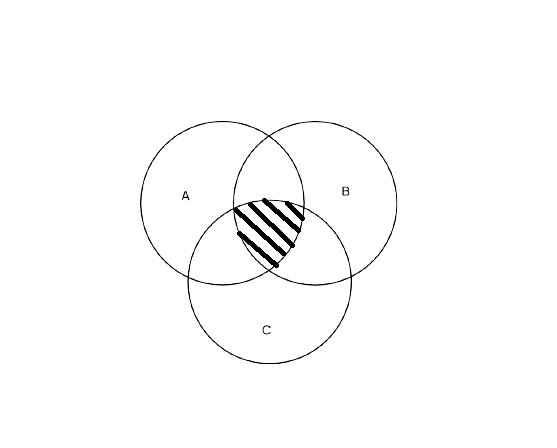
\includegraphics[width=0.5\textwidth]{latexvenn.png}
    \caption{Venn Diagram}
    \label{fig:my_label}
\end{figure}




{instead of labeling the shaded area, you can do the below!}

{Let the shaded area be } T

{From the Venn diagram, it can be seen that}

\begin{itemize}
    \item $(A \cap B) \cap (A \cap C) = T$
    \item $(B \cap B) \cap (B \cap C) = T$
    \item $(A \cap C) \cap (B \cap C) = T$
    \item $(A \cap B \cap C) = T$
\end{itemize}

{Therefore,}

$(A \cap B) \cap (A \cap C) = (A \cap B) \cap (B \cap C)
= (A \cap C) \cap (B \cap C) = A \cap B \cap C$



$= P(A \cap B) + P(A \cap C) + P(B \cap C) - P(A \cap B \cap C) - P(A \cap B \cap C) - P(A \cap B \cap C) + P(A \cap B \cap C)$
\\ \\
$= P(A \cap B) + P(A \cap C) + P(B \cap C) - 2P(A \cap B \cap C)$
\\ \\



\end{document}
